\usetikzlibrary{arrows,automata,positioning}
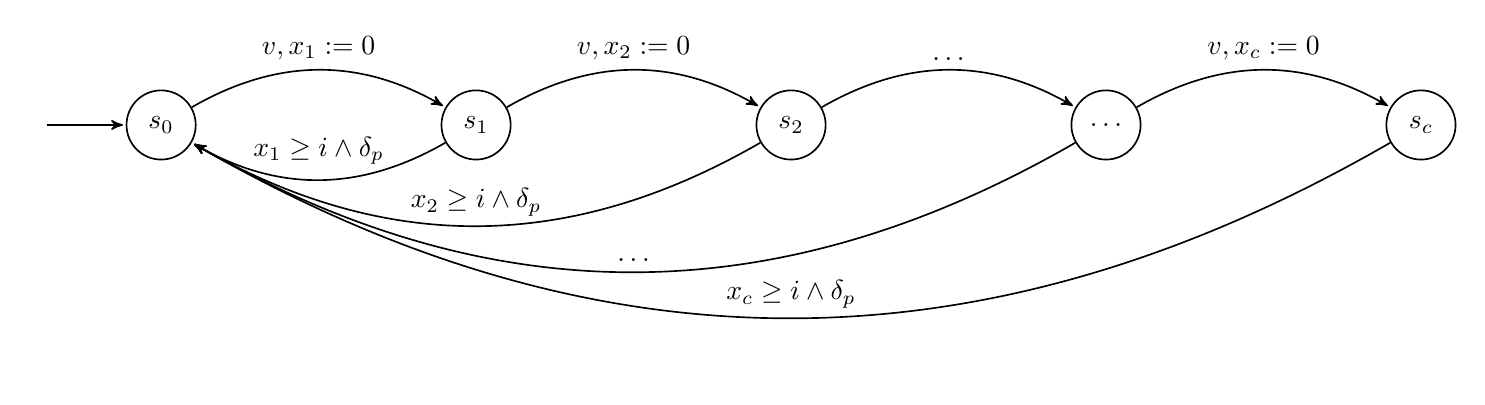
\begin{tikzpicture}[->,>=stealth',shorten >=1pt,auto,node distance=4cm, semithick]
	\node(start) {};
	\node[state] (S0) [right=0cm and 1cm of start]{$s_0$};
	\node[state] (S1) [right of=S0] {$s_1$};
	\node[state] (S2) [right of=S1] {$s_2$};
	\node[state] (Sd) [right of=S2] {$\dots$};
	\node[state] (Sc) [right of=Sd] {$s_c$};

	\path (start) edge node {} (S0);
	\path (S0) edge [bend left] node {$v, x_1 := 0$} (S1);
	\path (S1) edge [bend left] node [above=0.2em] {$x_1 \geq i \land \delta_p$} (S0);
	\path (S1) edge [bend left] node {$v, x_2 := 0$} (S2);
	\path (S2) edge [bend left] node [above] {$x_2 \geq i \land \delta_p$} (S0);
	\path (S2) edge [bend left] node {$\dots$} (Sd);
	\path (Sd) edge [bend left] node [above] {$\dots$} (S0);
	\path (Sd) edge [bend left] node {$v, x_c := 0$} (Sc);
	\path (Sc) edge [bend left] node [above] {$x_c \geq i \land \delta_p$} (S0);
\end{tikzpicture}
